% Provenance (never printed): cycle 4 SVT, "La planete Terre, l'environnement
% et l'action humaine": the relief as a balance between uplift and erosion;
% landforms of the wind, the sea and dissolution; reading a landscape; see
% sources/book1/PROVENANCE.md. Book 1, grade 9, chapter 4.
% Vocabulary guard: owns uplift, dune, cliff, beach and spit (with longshore
% drift), karst (with cave and sinkhole). Landscape and landform are g1's;
% weathering, erosion, deposition, meander and delta are g5's; relief is
% g4's; plates and mountain building are g7's; U-shaped valley and moraine
% are g8's; limestone and the acid test are g6's; acids are the chemistry
% books' (recalled in prose). Contour lines are g9.5's (not used here).
% "Normal fault" and the destruction of mountains are Book 2's.
\chapter{Landforms}\label{ch:g9:landforms}

On the south \omterm{def:g1:landscapes-around-us:water}{coast} of England, the white \omterm{def:g9:landforms:cliff}{cliffs} of the Seven Sisters drop
straight into the \omterm{def:g2:water-on-earth:ocean}{sea}. In a normal year they lose up to a metre. In the
winter of 2014, \omterm{def:g5:natural-hazards:storm}{storms} took from the \omterm{def:g9:landforms:cliff}{cliffs} at Birling Gap as much as they
usually lose in seven years, in two months. The chalk of these \omterm{def:g9:landforms:cliff}{cliffs} was
once \omterm{def:g3:stones-pebbles-sand:sand}{mud} on the floor of a \omterm{def:g2:water-on-earth:ocean}{sea}, made of the tiny plates of microscopic
algae that lived in its water. Today it stands as a wall of white \omterm{def:g3:stones-pebbles-sand:rock}{rock}
that the waves cut back a little further every year. Why does the land have
the shapes it has, and why do some of them change so fast?
% ledger: nt:birling-2014, sdnp:birling, nasa:coccoliths

\begin{omfigure}
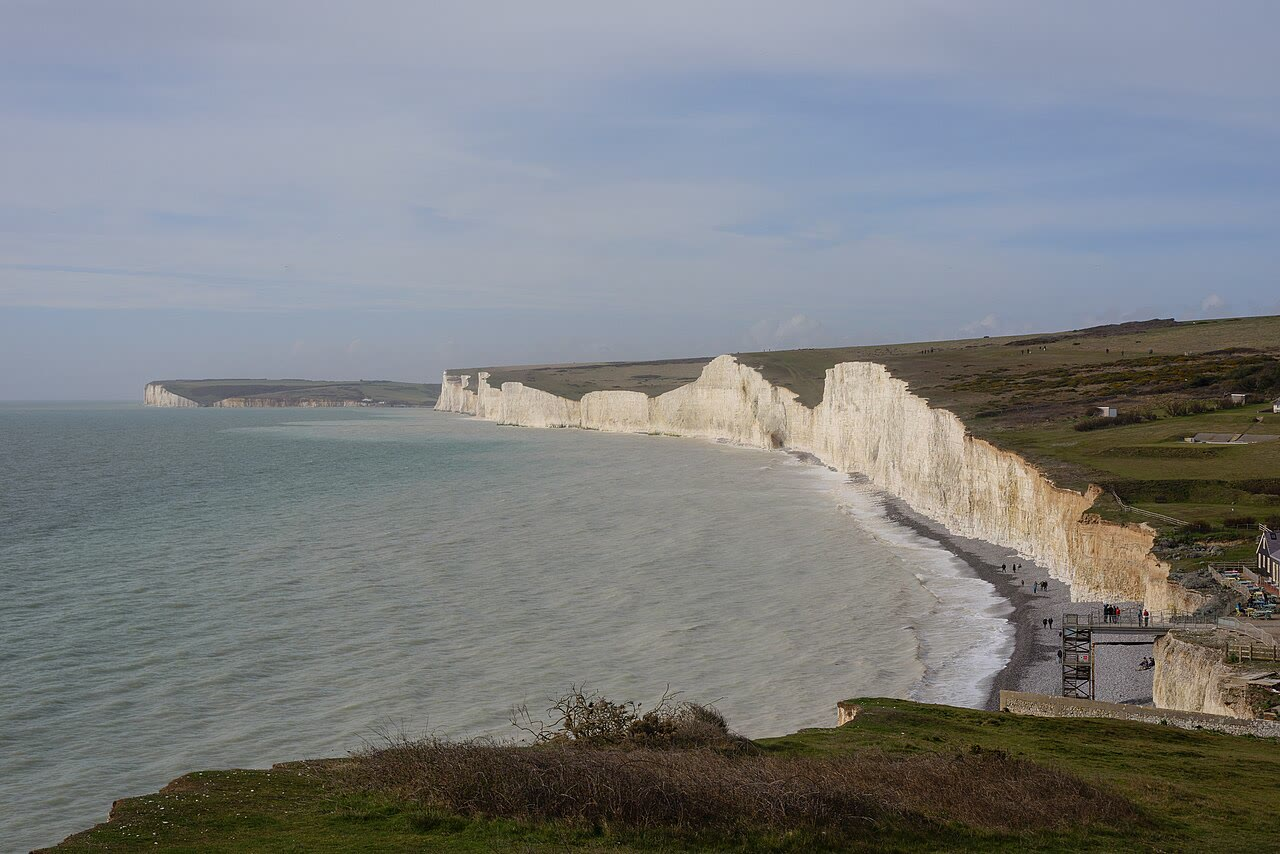
\includegraphics[width=\linewidth]{images/book1/g9-seven-sisters.jpg}

{\small The Seven Sisters, chalk \omterm{def:g9:landforms:cliff}{cliffs} on the \omterm{def:g1:landscapes-around-us:water}{coast} of East Sussex
(England), with the houses of Birling Gap in the foreground. The \omterm{def:g9:landforms:cliff}{cliffs}
are cut back by the \omterm{def:g2:water-on-earth:ocean}{sea}, and \omterm{def:g3:stones-pebbles-sand:rock}{rock} falls happen at any time. At their
foot lies a \omterm{def:g9:landforms:beach}{beach} of \omterm{def:g3:stones-pebbles-sand:pebble}{pebbles}. Photograph Arild Vågen, 2017 (CC BY-SA 4.0, via Wikimedia
Commons).}
% ledger: commons:seven-sisters, sdnp:birling
\label{fig:g9:landforms:seven-sisters}
\end{omfigure}

\begin{recall}
A \emph{\omterm{def:g1:landscapes-around-us:landform}{landform}} is one shape of the land: a \omterm{def:g1:landscapes-around-us:landform}{hill}, a \omterm{def:g1:landscapes-around-us:landform}{valley}, a \omterm{def:g1:landscapes-around-us:landform}{plain}, a
\omterm{def:g9:landforms:cliff}{cliff} (\cref{ch:g1:landscapes-around-us}). The \omterm{def:g4:world-physical-map:relief}{relief} is the shape of the
land in height (\cref{ch:g4:world-physical-map}). \omterm{def:g5:water-shapes-the-land:weathering}{Weathering} breaks the
\omterm{def:g3:stones-pebbles-sand:rock}{rock}, \omterm{def:g5:water-shapes-the-land:erosion}{erosion} wears it away and carries it off, and \omterm{def:g5:water-shapes-the-land:deposition}{deposition} lays it
down elsewhere (\cref{ch:g5:water-shapes-the-land}). The \omterm{def:g7:plate-tectonics:plate}{plates} push up
\omterm{def:g4:world-physical-map:range}{mountain ranges} where they collide (\cref{ch:g7:plate-tectonics}); \omterm{def:g8:ice-on-earth:glacier}{glaciers}
carve \omterm{def:g8:ice-on-earth:glacial-landforms}{U-shaped valleys} (\cref{ch:g8:ice-on-earth}); limestone fizzes under
a drop of dilute acid (\cref{ch:g6:rocks-and-minerals}). In chemistry, you
learn that acids attack limestone and give off carbon dioxide.
\end{recall}

\section{The relief: a balance between uplift and erosion}

Two kinds of forces shape the \omterm{def:g4:world-physical-map:relief}{relief}. From inside, the movements of the
\omterm{def:g7:plate-tectonics:plate}{plates} raise the ground. From outside, water, ice, wind and the \omterm{def:g2:water-on-earth:ocean}{sea} wear it
down.

\begin{definition}[Uplift]\label{def:g9:landforms:uplift}
\emph{Uplift}\index{uplift} is the slow rise of the \omterm{def:g3:stones-pebbles-sand:rock}{rocks} and the ground
surface of a region, driven by forces inside the Earth, such as the
collision of two \omterm{def:g7:plate-tectonics:plate}{plates}.
\end{definition}

\omterm{def:g9:landforms:uplift}{Uplift} is slow on the scale of a life but fast on the scale of the Earth.
India collided with Asia about 50~million years ago, and the Tibetan
Plateau, behind the Himalaya, gained most of its height, about
\qty{4600}{m}, in the last 10~million years. On average, that is
$4600 \div 10^7 = 4.6 \times 10^{-4}$~m, or about \qty{0.5}{mm} a year:
less than the thickness of a fingernail, but kept up for millions of years.
% ledger: usgs:himalaya (rate computed in figdata/grade-9/cliff_retreat.py, tibet_rate_mm_yr)

As soon as the ground rises, \omterm{def:g5:water-shapes-the-land:erosion}{erosion} attacks it. The higher and the
steeper the land, the faster \omterm{def:g1:landscapes-around-us:water}{rivers}, \omterm{def:g8:ice-on-earth:glacier}{glaciers} and \omterm{def:g3:stones-pebbles-sand:rock}{rock} falls carry \omterm{def:g3:stones-pebbles-sand:rock}{rock}
away. The height of a \omterm{def:g4:world-physical-map:range}{mountain range} at any moment is the result of a
contest: what \omterm{def:g9:landforms:uplift}{uplift} brings up, minus what \omterm{def:g5:water-shapes-the-land:erosion}{erosion} takes away.

\begin{omfigure}
\begin{tikzpicture}[font=\footnotesize, >={Stealth[length=2mm]}]
  % panel 1: uplift faster than erosion
  \begin{scope}
    \fill[black!13] (0,0) -- (0.5,0) .. controls (1.1,1.0) and (1.5,2.0) .. (1.8,2.2)
      .. controls (2.1,2.0) and (2.5,1.0) .. (3.1,0) -- (3.6,0) -- (3.6,-0.5) -- (0,-0.5) -- cycle;
    \draw[black!60] (0,0) -- (0.5,0) .. controls (1.1,1.0) and (1.5,2.0) .. (1.8,2.2)
      .. controls (2.1,2.0) and (2.5,1.0) .. (3.1,0) -- (3.6,0);
    \draw[black!60, dashed] (0.7,0) .. controls (1.2,0.8) and (1.5,1.5) .. (1.8,1.6)
      .. controls (2.1,1.5) and (2.4,0.8) .. (2.9,0);
    \foreach \x in {1.2,1.8,2.4} \draw[->, omWarm, line width=1.4pt] (\x,-0.45) -- ++(0,1.0);
    \draw[->, omRiver, thick] (2.15,1.6) -- ++(0.35,-0.3);
    \node[align=center, anchor=north] at (1.8,-0.6) {uplift faster than erosion:\\the relief rises};
  \end{scope}
  % panel 2: uplift equals erosion
  \begin{scope}[xshift=4.4cm]
    \fill[black!13] (0,0) -- (0.5,0) .. controls (1.1,1.0) and (1.5,1.8) .. (1.8,1.9)
      .. controls (2.1,1.8) and (2.5,1.0) .. (3.1,0) -- (3.6,0) -- (3.6,-0.5) -- (0,-0.5) -- cycle;
    \draw[black!60] (0,0) -- (0.5,0) .. controls (1.1,1.0) and (1.5,1.8) .. (1.8,1.9)
      .. controls (2.1,1.8) and (2.5,1.0) .. (3.1,0) -- (3.6,0);
    \foreach \x in {1.2,1.8,2.4} \draw[->, omWarm, line width=1.4pt] (\x,-0.45) -- ++(0,0.6);
    \draw[->, omRiver, thick] (2.05,1.6) -- ++(0.55,-0.5);
    \draw[->, omRiver, thick] (1.55,1.6) -- ++(-0.55,-0.5);
    \node[align=center, anchor=north] at (1.8,-0.6) {uplift and erosion equal:\\the height stays the same};
  \end{scope}
  % panel 3: no more uplift
  \begin{scope}[xshift=8.8cm]
    \fill[black!13] (0,0) -- (0.4,0) .. controls (1.1,0.5) and (1.5,0.95) .. (1.8,1.0)
      .. controls (2.1,0.95) and (2.5,0.5) .. (3.2,0) -- (3.6,0) -- (3.6,-0.5) -- (0,-0.5) -- cycle;
    \draw[black!60] (0,0) -- (0.4,0) .. controls (1.1,0.5) and (1.5,0.95) .. (1.8,1.0)
      .. controls (2.1,0.95) and (2.5,0.5) .. (3.2,0) -- (3.6,0);
    \draw[black!60, dashed] (0.5,0) .. controls (1.1,1.0) and (1.5,1.8) .. (1.8,1.9)
      .. controls (2.1,1.8) and (2.5,1.0) .. (3.1,0);
    \draw[->, omRiver, thick] (2.05,0.95) -- ++(0.55,-0.5);
    \draw[->, omRiver, thick] (1.55,0.95) -- ++(-0.55,-0.5);
    \node[align=center, anchor=north] at (1.8,-0.6) {no more uplift: erosion\\lowers the relief};
  \end{scope}
  % key
  \draw[->, omWarm, line width=1.4pt] (13.2,1.2) -- ++(0,0.6) node[right, black] {uplift};
  \draw[->, omRiver, thick] (13.2,0.7) -- ++(0.35,-0.3) node[right, black] {erosion};
  \draw[black!60, dashed] (13.1,-0.1) -- ++(0.5,0) node[right, black] {earlier profile};
\end{tikzpicture}

{\small The \omterm{def:g4:world-physical-map:relief}{relief} as a balance (a sketch, not to scale). \omterm{def:g9:landforms:uplift}{Uplift} raises the
\omterm{def:g3:stones-pebbles-sand:rock}{rocks}; \omterm{def:g5:water-shapes-the-land:erosion}{erosion} carries them away to the \omterm{def:g1:landscapes-around-us:landform}{valleys} and the \omterm{def:g2:water-on-earth:ocean}{sea}. A range keeps
growing as long as \omterm{def:g9:landforms:uplift}{uplift} wins; when the \omterm{def:g7:plate-tectonics:plate}{plates} stop pushing, \omterm{def:g5:water-shapes-the-land:erosion}{erosion} slowly
wears it down to \omterm{def:g1:landscapes-around-us:landform}{hills}.}
\label{fig:g9:landforms:balance}
\end{omfigure}

\omterm{def:g1:landscapes-around-us:water}{Rivers} (\cref{ch:g5:water-shapes-the-land}) and \omterm{def:g8:ice-on-earth:glacier}{glaciers}
(\cref{ch:g8:ice-on-earth}) are the great carvers of \omterm{def:g1:landscapes-around-us:landform}{mountains}. The rest of
this chapter follows three other agents, which make \omterm{def:g1:landscapes-around-us:landform}{landforms} of their
own: the wind, the \omterm{def:g2:water-on-earth:ocean}{sea}, and water that dissolves \omterm{def:g3:stones-pebbles-sand:rock}{rock}.

\section{Landforms made by the wind: dunes}

Where plants are few, loose \omterm{def:g3:stones-pebbles-sand:sand}{sand} plentiful and the wind strong, the wind
can pick up \omterm{def:g3:stones-pebbles-sand:sand}{sand} and heap it into \omterm{def:g1:landscapes-around-us:landform}{hills}: in \omterm{def:g5:weather-and-climate:desert}{deserts}, and behind sandy
\omterm{def:g9:landforms:beach}{beaches}.
% ledger: nps:aeolian

\begin{definition}[Dune]\label{def:g9:landforms:dune}
A \emph{dune}\index{dune} is a mound or ridge of loose \omterm{def:g3:stones-pebbles-sand:sand}{sand} heaped up by
the wind. Its slope facing the wind is long and gentle; its far side, the
\emph{slip face}\index{slip face}, is short and steep.
\end{definition}
% ledger: nps:aeolian, nmt:barchan

A \omterm{def:g9:landforms:dune}{dune} moves. The wind rolls and bounces the grains up the gentle slope;
at the crest they pile up until the heap becomes too steep, and a little
avalanche of \omterm{def:g3:stones-pebbles-sand:sand}{sand} slides down the \omterm{def:g9:landforms:dune}{slip face}. Grain after grain, \omterm{def:g3:stones-pebbles-sand:sand}{sand} is
taken from the windward side and laid on the far side, and the whole \omterm{def:g9:landforms:dune}{dune}
creeps downwind without ever being lifted. \omterm{def:g9:landforms:dune}{Dunes} rarely stand alone: they
cover whole fields.
% ledger: nmt:barchan, nps:aeolian

Where the wind always blows from the same direction and \omterm{def:g3:stones-pebbles-sand:sand}{sand} is not too
plentiful, \omterm{def:g9:landforms:dune}{dunes} take the shape of a crescent, a \emph{barchan}: its round
nose faces the wind and its two horns point downwind. The horns hold less
\omterm{def:g3:stones-pebbles-sand:sand}{sand} than the middle, so they move faster and stretch ahead of the \omterm{def:g9:landforms:dune}{dune}.
% ledger: nmt:barchan

\begin{omfigure}
\begin{tikzpicture}[font=\footnotesize, >={Stealth[length=2mm]}]
  % plan view
  \fill[yellow!25!orange!20] (3.4,1.3) .. controls (1.0,1.3) and (0.2,0.6) .. (0.2,0)
     .. controls (0.2,-0.6) and (1.0,-1.3) .. (3.4,-1.3)
     .. controls (2.4,-0.9) and (1.8,-0.5) .. (1.8,0)
     .. controls (1.8,0.5) and (2.4,0.9) .. (3.4,1.3) -- cycle;
  \fill[orange!45] (3.4,1.3) .. controls (2.4,0.9) and (1.8,0.5) .. (1.8,0)
     .. controls (1.8,-0.5) and (2.4,-0.9) .. (3.4,-1.3)
     .. controls (2.1,-0.8) and (1.45,-0.45) .. (1.45,0)
     .. controls (1.45,0.45) and (2.1,0.8) .. (3.4,1.3) -- cycle;
  \draw[black!60] (3.4,1.3) .. controls (1.0,1.3) and (0.2,0.6) .. (0.2,0)
     .. controls (0.2,-0.6) and (1.0,-1.3) .. (3.4,-1.3)
     .. controls (2.4,-0.9) and (1.8,-0.5) .. (1.8,0)
     .. controls (1.8,0.5) and (2.4,0.9) .. (3.4,1.3);
  \draw[black, thick] (3.4,1.3) .. controls (2.1,0.8) and (1.45,0.45) .. (1.45,0)
     .. controls (1.45,-0.45) and (2.1,-0.8) .. (3.4,-1.3);
  \foreach \y in {-0.8,0,0.8} \draw[->, omRiver, thick] (-1.3,\y) -- ++(1.1,0);
  \node[above] at (-0.75,0.85) {wind};
  \node[anchor=west] at (3.5,1.35) {horn};
  \node[anchor=west] at (3.5,-1.35) {horn};
  \draw[black!70] (1.75,0.25) -- (2.9,0.35) node[anchor=west, align=left, black] {slip face\\(steep)};
  \draw[black!70] (0.75,-0.2) -- (0.6,-1.6) node[anchor=north, align=center, black] {windward slope\\(gentle)};
  \draw[black!70] (1.47,-0.3) -- (2.4,-1.75) node[anchor=north, black] {crest};
  \node[anchor=south, font=\footnotesize\bfseries] at (1.4,1.6) {seen from above};
  % profile
  \begin{scope}[xshift=7.2cm, yshift=-0.8cm]
    \draw[black!60] (-0.4,0) -- (5.6,0);
    \fill[yellow!25!orange!20] (0,0) -- (3.0,1.2) -- (3.6,0) -- cycle;
    \draw[black!70] (0,0) -- (3.0,1.2) -- (3.6,0);
    \fill[orange!45] (3.0,1.2) -- (3.6,0) -- (3.3,0) -- cycle;
    \draw[black!50, dashed] (0.8,0) -- (3.8,1.2) -- (4.4,0);
    \draw[->, black!70] (0.5,0.35) .. controls (0.75,0.65) .. (1.0,0.45);
    \draw[->, black!70] (1.0,0.55) .. controls (1.25,0.85) .. (1.5,0.65);
    \draw[->, black!70] (1.5,0.75) .. controls (1.75,1.05) .. (2.0,0.85);
    \draw[->, black!70] (2.0,0.95) .. controls (2.25,1.25) .. (2.5,1.05);
    \draw[->, thick, black!80] (3.15,1.05) -- (3.45,0.35);
    \foreach \y in {1.6,2.1} \draw[->, omRiver, thick] (-0.8,\y) -- ++(1.1,0);
    \node[above] at (-0.25,2.1) {wind};
    \draw[->, thick] (4.5,0.6) -- ++(0.7,0) node[right, align=left] {the dune\\moves};
    \node[align=center, anchor=north] at (1.2,-0.1) {grains bounce up\\the gentle slope};
    \node[align=center, anchor=north west] at (2.9,-0.1) {and slide down\\the slip face};
    \node[anchor=south, font=\footnotesize\bfseries] at (2.2,2.3) {seen from the side};
  \end{scope}
\end{tikzpicture}

{\small A crescent \omterm{def:g9:landforms:dune}{dune}, or barchan (a sketch). Seen from above, its horns
point downwind. Seen from the side, the grains climb the gentle windward
slope and slide down the steep \omterm{def:g9:landforms:dune}{slip face}: the \omterm{def:g9:landforms:dune}{dune} moves downwind (dashed
outline: the \omterm{def:g9:landforms:dune}{dune} a little later).}
% ledger: nmt:barchan, nps:aeolian
\label{fig:g9:landforms:barchan}
\end{omfigure}

How fast? In the gypsum \omterm{def:g9:landforms:dune}{dune} field of White Sands, in New Mexico, the
small \omterm{def:g9:landforms:dune}{dunes} that form at its upwind edge, a few metres high, move up to
\qty{6}{m} a year; a little further on, grown to 6 to \qty{10}{m} high,
they move about \qty{3}{m} a year. The more \omterm{def:g3:stones-pebbles-sand:sand}{sand} a \omterm{def:g9:landforms:dune}{dune} holds, the slower
it goes. Barchans driven by strong winds can travel more than \qty{100}{m}
in a year, enough to bury a road or a field.
% ledger: nps:whsa-migration, nmt:barchan

\begin{omfigure}
\begin{minipage}[c]{0.5\linewidth}\centering
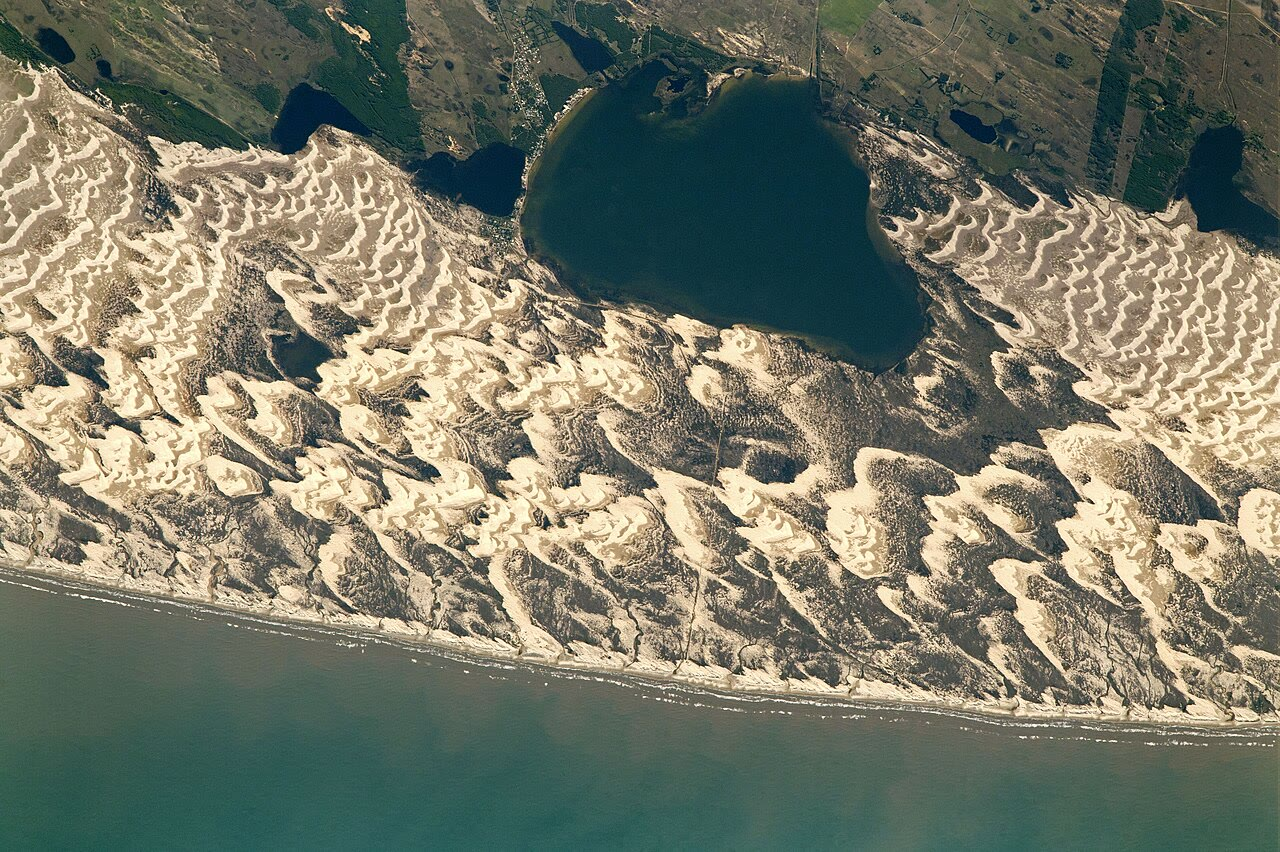
\includegraphics[width=\linewidth]{images/book1/g9-barchans.jpg}
\end{minipage}\hfill
\begin{minipage}[c]{0.46\linewidth}\raggedright
{\small Crescent-shaped \omterm{def:g9:landforms:dune}{dunes} on the Atlantic \omterm{def:g1:landscapes-around-us:water}{coast} of southern Brazil,
photographed by an astronaut from the International Space Station in 2017.
The dark \omterm{def:g1:landscapes-around-us:water}{lake}, Lagoa dos Barros, is about \qty{4.5}{km} long. The \omterm{def:g3:stones-pebbles-sand:sand}{sand}
comes from the \omterm{def:g9:landforms:beach}{beach}, at the bottom of the photograph. NASA (public domain,
via Wikimedia Commons).}
\end{minipage}
% ledger: commons:iss-barchans
\label{fig:g9:landforms:barchans-photo}
\end{omfigure}

On a \omterm{def:g1:landscapes-around-us:water}{coast}, a line of \omterm{def:g9:landforms:dune}{dunes} behind the \omterm{def:g9:landforms:beach}{beach} shields the land behind it
from \omterm{def:g5:natural-hazards:storm}{storm} waves. Plants that grow on the \omterm{def:g9:landforms:dune}{dunes} hold the \omterm{def:g3:stones-pebbles-sand:sand}{sand} with their
roots: where they are trampled or cleared, the wind takes the \omterm{def:g3:stones-pebbles-sand:sand}{sand} again.
% ledger: nps:aeolian

\section{Landforms made by the sea}

\subsection{Cliffs}

\begin{definition}[Cliff]\label{def:g9:landforms:cliff}
A \emph{cliff}\index{cliff} is a steep or vertical face of \omterm{def:g3:stones-pebbles-sand:rock}{rock}. On a
\omterm{def:g1:landscapes-around-us:water}{coast}, a cliff is cut by the waves, which attack its foot and make it
retreat inland.
\end{definition}

Waves hurl water, \omterm{def:g3:stones-pebbles-sand:sand}{sand} and \omterm{def:g3:stones-pebbles-sand:pebble}{pebbles} at the foot of the \omterm{def:g9:landforms:cliff}{cliff}. Little by
little they cut a hollow at its base, a \emph{notch}, between the levels of
low and high tide. The \omterm{def:g3:stones-pebbles-sand:rock}{rock} above overhangs; \omterm{def:g4:clouds-rain-snow:precipitation}{rain} and frost weaken it
further. One day the overhang falls. The waves break up the fallen blocks
and carry them away, and the attack starts again on a fresh face, a little
further inland. Behind it, the \omterm{def:g9:landforms:cliff}{cliff} leaves a flat shelf of \omterm{def:g3:stones-pebbles-sand:rock}{rock}, the
\emph{wave-cut platform}\index{wave-cut platform}, which appears at low
tide.
% ledger: nt:birling-2014, sdnp:birling

Soft \omterm{def:g3:stones-pebbles-sand:rock}{rocks} retreat fastest. At Birling Gap, the chalk \omterm{def:g9:landforms:cliff}{cliffs} lose up to
about a metre a year; but the retreat comes in jumps, one fall at a time,
and a stormy winter can take years of retreat at once. In 1999, the old
Belle Tout lighthouse, built in 1832 on top of the \omterm{def:g9:landforms:cliff}{cliffs} nearby, was moved
\qty{17}{m} back from the edge, in one piece, because the \omterm{def:g9:landforms:cliff}{cliff} was coming
too close.
% ledger: sdnp:birling, nt:birling-2014

\begin{omfigure}
\begin{tikzpicture}[font=\footnotesize, >={Stealth[length=2mm]}]
  % panel 1: the notch
  \begin{scope}
    \fill[omSea!45] (0,-0.1) rectangle (1.8,0.75);
    \fill[omSea!45] (1.8,0.35) -- (2.25,0.55) -- (1.8,0.95) -- cycle;
    \fill[black!8] (1.6,-0.1) -- (1.8,0.25) -- (1.8,0.35) -- (2.25,0.55) -- (1.8,0.95) -- (1.8,2.4) -- (3.6,2.4) -- (3.6,-0.6) -- (0,-0.6) -- (0,-0.1) -- cycle;
    \draw[black!70] (0,-0.1) -- (1.6,-0.1) -- (1.8,0.25) -- (1.8,0.35) -- (2.25,0.55) -- (1.8,0.95) -- (1.8,2.4) -- (3.6,2.4);
    \foreach \y in {0.8,1.3,1.8} \draw[black!25] (1.8,\y) -- (3.6,\y);
    \fill[green!35!black!50] (1.8,2.4) rectangle (3.6,2.5);
    \draw[->, omSea!80!black, thick] (0.4,0.6) -- (1.6,0.6);
    \node[anchor=south, align=center] at (0.9,0.8) {waves};
    \draw[black!70] (2.15,0.55) -- (2.9,1.0) node[anchor=west, fill=white, inner sep=1pt] {notch};
    \node[anchor=north, align=center] at (1.8,-0.7) {1. the waves cut\\a notch};
    \node[anchor=south, font=\footnotesize] at (2.7,2.5) {chalk};
  \end{scope}
  % panel 2: collapse
  \begin{scope}[xshift=4.6cm]
    \fill[omSea!45] (0,-0.1) rectangle (2.2,0.75);
    \fill[black!8] (2.0,-0.1) -- (2.2,0.25) -- (2.25,2.4) -- (3.6,2.4) -- (3.6,-0.6) -- (0,-0.6) -- (0,-0.1) -- cycle;
    \draw[black!70] (0,-0.1) -- (2.0,-0.1) -- (2.2,0.25) -- (2.25,2.4) -- (3.6,2.4);
    \draw[black!50, dashed] (1.8,0.95) -- (1.8,2.4) -- (2.25,2.4);
    \foreach \y in {0.8,1.3,1.8} \draw[black!25] (2.25,\y) -- (3.6,\y);
    \fill[green!35!black!50] (2.25,2.4) rectangle (3.6,2.5);
    \foreach \x/\y/\s in {1.25/0.05/0.28, 1.6/0.1/0.22, 1.95/0.3/0.3, 1.45/0.35/0.18}
      \fill[black!20, draw=black!60] (\x,\y) rectangle ++(\s,\s*0.8);
    \node[anchor=north, align=center] at (1.8,-0.7) {2. the overhang\\falls};
  \end{scope}
  % panel 3: retreat and platform
  \begin{scope}[xshift=9.2cm]
    \fill[omSea!45] (0,0.2) rectangle (2.8,0.75);
    \fill[black!8] (0,0.0) -- (2.6,0.2) -- (2.8,0.3) -- (2.85,2.4) -- (4.0,2.4) -- (4.0,-0.6) -- (0,-0.6) -- cycle;
    \draw[black!70] (0,0.0) -- (2.6,0.2) -- (2.8,0.3) -- (2.85,2.4) -- (4.0,2.4);
    \foreach \y in {0.8,1.3,1.8} \draw[black!25] (2.85,\y) -- (4.0,\y);
    \fill[green!35!black!50] (2.85,2.4) rectangle (4.0,2.5);
    \draw[black!50, dashed] (1.4,0.12) -- (1.4,2.4);
    \draw[black!50, dashed] (2.1,0.16) -- (2.1,2.4);
    \draw[<-, thick] (2.8,1.6) -- (1.5,1.6);
    \node[anchor=south, align=center] at (1.4,2.45) {old cliff faces};
    \node[anchor=north, align=center] at (2.0,-0.7) {3. a wave-cut platform,\\uncovered at low tide};
  \end{scope}
\end{tikzpicture}

{\small How a \omterm{def:g2:water-on-earth:ocean}{sea} \omterm{def:g9:landforms:cliff}{cliff} retreats (a sketch, not to scale). (1) The waves
cut a notch at the foot of the \omterm{def:g9:landforms:cliff}{cliff}. (2) The overhanging \omterm{def:g3:stones-pebbles-sand:rock}{rock} falls; the
waves break up the blocks and carry them away. (3) The cycle repeats: the
\omterm{def:g9:landforms:cliff}{cliff} moves inland and leaves a flat \omterm{def:g3:stones-pebbles-sand:rock}{rock} platform in front of it.}
% ledger: nt:birling-2014, sdnp:birling
\label{fig:g9:landforms:cliff-retreat}
\end{omfigure}

\begin{safety}
The edge of a \omterm{def:g9:landforms:cliff}{cliff} can give way at any moment, and \omterm{def:g3:stones-pebbles-sand:rock}{rocks} fall from the
face without warning. \omterm{def:g9:landforms:cliff}{Cliffs} are watched from a safe distance, well back
from the edge at the top and well away from the foot on the \omterm{def:g9:landforms:beach}{beach}, and a
\omterm{def:g9:landforms:beach}{beach} below \omterm{def:g9:landforms:cliff}{cliffs} is left before the tide comes in.
\end{safety}
% ledger: nt:birling-2014, sdnp:birling

\subsection{Beaches and spits}

The \omterm{def:g3:stones-pebbles-sand:sand}{sand} and \omterm{def:g3:stones-pebbles-sand:pebble}{pebbles} worn from \omterm{def:g9:landforms:cliff}{cliffs}, and brought down by \omterm{def:g1:landscapes-around-us:water}{rivers}, do not
stay where they fall: the waves sort them and move them along the \omterm{def:g1:landscapes-around-us:water}{coast}.

\begin{definition}[Beach, longshore drift and spit]\label{def:g9:landforms:beach}
A \emph{beach}\index{beach} is a strip of \omterm{def:g3:stones-pebbles-sand:sand}{sand} or \omterm{def:g3:stones-pebbles-sand:pebble}{pebbles} piled up by the
waves along the shore. When the waves reach the shore at an angle, each
wave pushes the grains up the beach at that angle and the water runs back
straight down the slope: the grains zigzag along the \omterm{def:g1:landscapes-around-us:water}{coast}. This movement
of \omterm{def:g3:stones-pebbles-sand:sand}{sand} and \omterm{def:g3:stones-pebbles-sand:pebble}{pebbles} along the shore is \emph{longshore
drift}\index{longshore drift}. A \emph{spit}\index{spit} is a long, narrow
ridge of \omterm{def:g3:stones-pebbles-sand:sand}{sand} or \omterm{def:g3:stones-pebbles-sand:pebble}{pebbles} built by longshore drift, joined to the land at
one end and running out into the \omterm{def:g2:water-on-earth:ocean}{sea} where the \omterm{def:g1:landscapes-around-us:water}{coast} turns.
\end{definition}
% ledger: noaa:longshore

Where the \omterm{def:g1:landscapes-around-us:water}{coast} bends, at the mouth of a bay or of a \omterm{def:g1:landscapes-around-us:water}{river}, the drift
carries on in the same direction and drops its load in the calmer water:
the \omterm{def:g9:landforms:beach}{beach} grows out into the \omterm{def:g2:water-on-earth:ocean}{sea} as a \omterm{def:g9:landforms:beach}{spit}. Its end often curls inward,
bent by waves coming from other directions. Behind the \omterm{def:g9:landforms:beach}{spit}, sheltered
from the waves, \omterm{def:g3:stones-pebbles-sand:sand}{mud} settles and salt marshes grow.
% ledger: noaa:longshore

\begin{omfigure}
\begin{tikzpicture}[font=\footnotesize, >={Stealth[length=2mm]}]
  % sea
  \fill[omSea!40] (0,0) rectangle (11,2.3);
  % land with a bay
  \fill[green!25!black!20] (0,2.3) -- (6,2.3) .. controls (6.3,3.0) and (7.0,3.5) .. (8.0,3.5)
     .. controls (9.0,3.5) and (9.3,2.8) .. (9.5,2.3) -- (11,2.3) -- (11,4.6) -- (0,4.6) -- cycle;
  % calm water of the bay
  \fill[omSea!20] (6,2.3) .. controls (6.3,3.0) and (7.0,3.5) .. (8.0,3.5)
     .. controls (9.0,3.5) and (9.3,2.8) .. (9.5,2.3) -- cycle;
  % salt marsh
  \fill[green!50!black!35] (6.15,2.55) .. controls (6.6,3.1) and (7.3,3.2) .. (7.9,3.0)
     .. controls (7.6,2.7) and (7.0,2.6) .. (6.15,2.55) -- cycle;
  \node[anchor=west, font=\scriptsize] at (6.5,3.85) {salt marsh};
  \draw[black!60] (6.9,3.75) -- (7.0,2.95);
  % river
  \draw[omRiver, line width=1.2pt] (8.6,4.6) .. controls (8.5,4.0) and (8.3,3.7) .. (8.3,3.48);
  \node[anchor=west, font=\scriptsize] at (8.65,4.25) {river};
  % beach
  \fill[yellow!40!orange!35] (0,1.85) rectangle (6,2.3);
  % spit
  \fill[yellow!40!orange!35] (5.9,1.85) .. controls (7.0,1.95) and (7.8,2.0) .. (8.35,2.1)
     .. controls (8.6,2.2) and (8.6,2.5) .. (8.4,2.65) -- (8.25,2.55)
     .. controls (8.35,2.45) and (8.3,2.35) .. (8.15,2.32)
     .. controls (7.5,2.28) and (6.8,2.3) .. (6.0,2.3) -- cycle;
  \draw[black!60] (0,2.3) -- (6,2.3) .. controls (6.3,3.0) and (7.0,3.5) .. (8.0,3.5)
     .. controls (9.0,3.5) and (9.3,2.8) .. (9.5,2.3) -- (11,2.3);
  % waves arriving at an angle
  \foreach \x in {0.9,2.0,3.1,4.2} \draw[omSea!70!black, line width=0.5pt] (\x,1.15) -- ++(-35:1.1);
  \draw[->, omSea!70!black, thick] (0.6,0.3) -- ++(55:1.2) node[pos=0.15, left, black] {waves};
  % zigzag of a pebble
  \draw[->, black, thick] (1.0,1.9) -- (1.35,2.2) -- (1.35,1.9) -- (1.7,2.2) -- (1.7,1.9)
     -- (2.05,2.2) -- (2.05,1.9) -- (2.4,2.2) -- (2.4,1.9);
  \node[anchor=south, align=center, font=\scriptsize] at (1.7,2.45) {up the beach at\\an angle, back\\straight down};
  % drift arrow
  \draw[->, line width=1.6pt, omWarm] (3.0,1.55) -- (5.6,1.55) node[midway, below, black] {longshore drift};
  % spit label
  \draw[black!70] (7.4,2.05) -- (7.6,1.2) node[anchor=north, align=center, black] {the spit grows\\across the bay};
  \draw[->, thick, omWarm] (8.6,1.95) -- ++(0.6,0);
  % compass
  \draw[->] (10.4,0.3) -- ++(0,0.6) node[above] {N};
\end{tikzpicture}

{\small \omterm{def:g9:landforms:beach}{Longshore drift} and a \omterm{def:g9:landforms:beach}{spit}, seen from above (a sketch). The waves
arrive from the south-west; each one pushes the \omterm{def:g3:stones-pebbles-sand:sand}{sand} and \omterm{def:g3:stones-pebbles-sand:pebble}{pebbles} up the
\omterm{def:g9:landforms:beach}{beach} at an angle, and the water runs back straight down: the grains zigzag
eastward. Where the \omterm{def:g1:landscapes-around-us:water}{coast} turns into a bay, the drift carries on and builds
a \omterm{def:g9:landforms:beach}{spit}, behind which a salt marsh grows. The \omterm{def:g1:landscapes-around-us:water}{river} keeps a channel open at
the end of the \omterm{def:g9:landforms:beach}{spit}.}
% ledger: noaa:longshore
\label{fig:g9:landforms:spit}
\end{omfigure}

\begin{omfigure}
\begin{minipage}[c]{0.5\linewidth}\centering
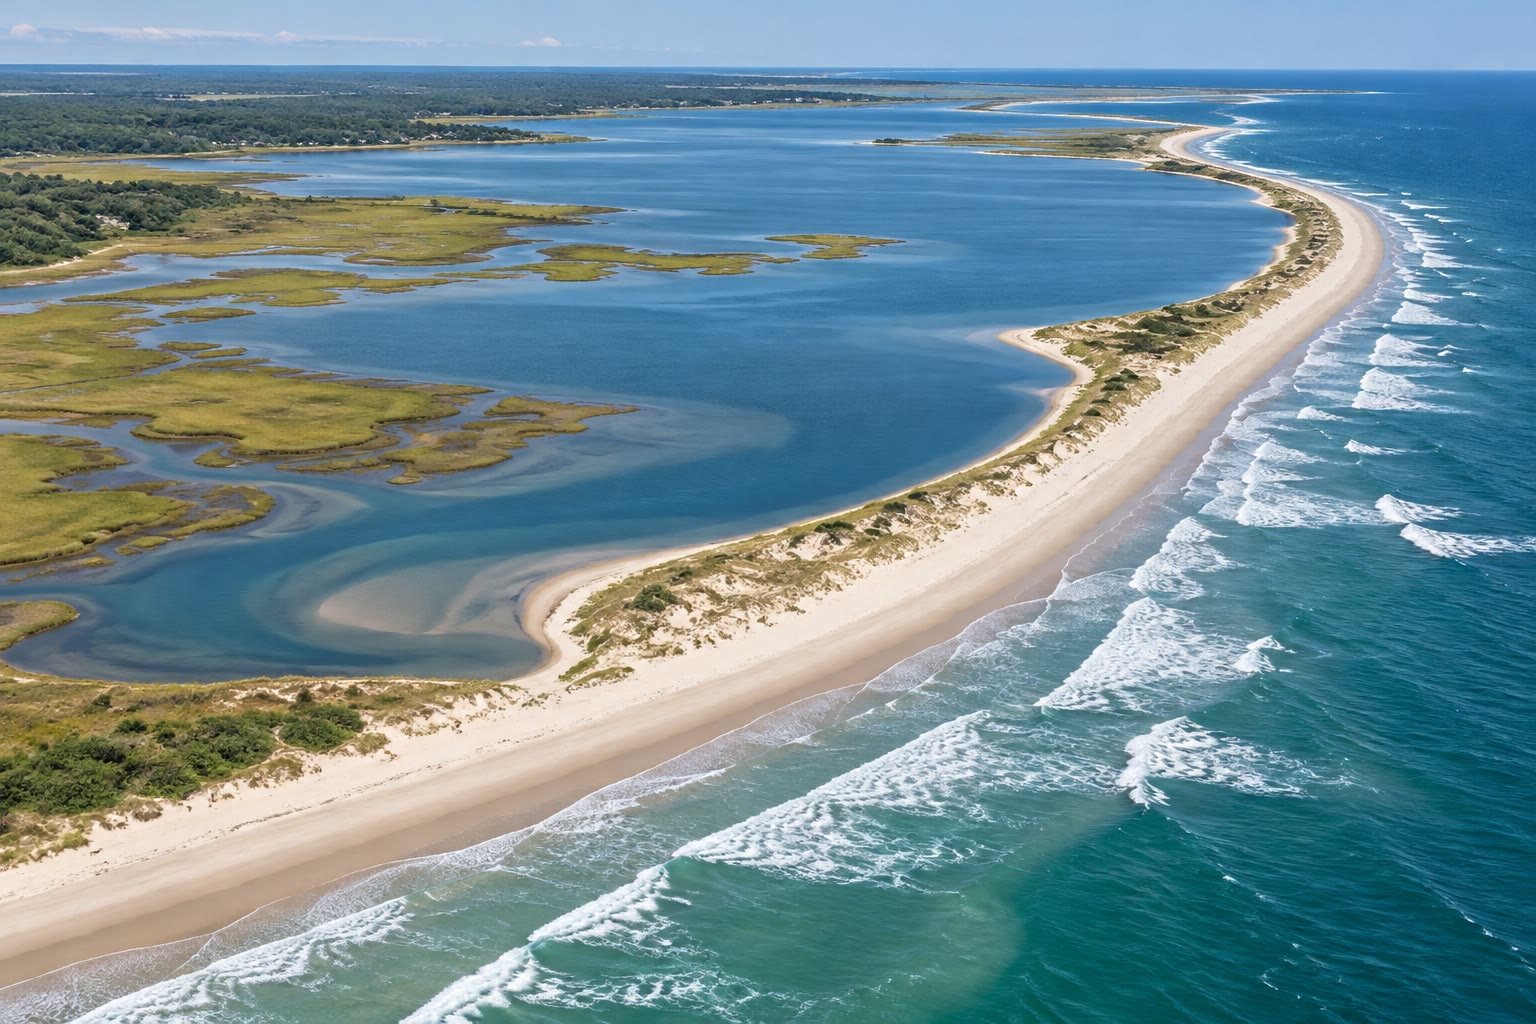
\includegraphics[width=\linewidth]{images/book1/ai/g9-spit-aerial.jpg}
\end{minipage}\hfill
\begin{minipage}[c]{0.46\linewidth}\raggedright
{\small A sandy \omterm{def:g9:landforms:beach}{spit} across the mouth of a bay, seen from a low aircraft
(an illustration, not a real place). The waves break on its seaward
\omterm{def:g9:landforms:beach}{beach}; behind it lie calm water and salt marshes.}
\end{minipage}
\label{fig:g9:landforms:spit-ai}
\end{omfigure}

\section{Landforms made by dissolution: karst}

Rainwater is not pure water. Falling through the air and then soaking
through the soil, it takes up carbon dioxide, which makes it slightly
acidic. This weak acid does slowly what the drop of dilute acid does fast
to a piece of limestone: it dissolves the \omterm{def:g3:stones-pebbles-sand:rock}{rock}. Limestone is full of
cracks, along its layers and across them. Water seeps down them and widens
them, millimetre by millimetre, over thousands of years.
% ledger: usgs:sinkholes, nps:karst

\begin{definition}[Karst, cave and sinkhole]\label{def:g9:landforms:karst}
A \emph{karst}\index{karst} is a \omterm{def:g1:landscapes-around-us:landscape}{landscape} shaped by water dissolving a
soluble \omterm{def:g3:stones-pebbles-sand:rock}{rock}, most often limestone. \omterm{def:g1:landscapes-around-us:water}{Rivers} there tend to vanish
underground and come back out as \omterm{def:g6:water-underground:spring}{springs}. A \emph{cave}\index{cave} is a
natural underground space large enough for a person to enter, dissolved
along the cracks of the \omterm{def:g3:stones-pebbles-sand:rock}{rock}. A \emph{sinkhole}\index{sinkhole} is a hollow
or a hole in the ground surface, formed where the \omterm{def:g3:stones-pebbles-sand:rock}{rock} below dissolves
away or where the roof of a cave collapses.
\end{definition}
% ledger: nps:karst, usgs:sinkholes

\begin{omfigure}
\begin{tikzpicture}[x=0.9cm, y=0.9cm, font=\footnotesize, >={Stealth[length=2mm]}]
  \pic (B) at (0,0) {blockdiagram={10}{4}{4}};
  % top face: grassland
  \fill[green!25!black!18] (B-ftl) -- (B-ftr) -- (B-btr) -- (B-btl) -- cycle;
  % right face
  \fill[omLithLime!70] (B-fbr) -- (B-bbr) -- (B-btr) -- (B-ftr) -- cycle;
  % front face: limestone layers
  \fill[omLithLime] (B-fbl) rectangle (B-ftr);
  \foreach \y in {0.8,1.6,2.4,3.2} \draw[black!35] (0,\y) -- (10,\y);
  \foreach \x/\y in {1.2/0.8, 3.1/1.6, 4.6/0, 6.8/2.4, 8.3/0.8, 2.2/2.4, 9.1/2.4, 5.6/3.2}
    \draw[black!35] (\x,\y) -- ++(0,0.8);
  % soil
  \fill[brown!45] (0,3.8) rectangle (10,4);
  % sinkhole on the top face and in the front face
  \fill[green!25!black!35] (3.0,4.45) ellipse (0.7 and 0.22);
  \fill[white] (2.3,4) -- (3.7,4) -- (3.25,3.45) -- (2.75,3.45) -- cycle;
  \fill[green!25!black!30] (2.3,4) -- (3.7,4) -- (3.25,3.45) -- (2.75,3.45) -- cycle;
  \draw[black!60] (2.3,4) -- (2.75,3.45) -- (3.25,3.45) -- (3.7,4);
  % shaft from sinkhole to cave
  \fill[white] (2.85,3.45) -- (3.15,3.45) -- (3.35,2.0) -- (3.05,2.0) -- cycle;
  \draw[black!60] (2.85,3.45) -- (3.05,2.0) (3.15,3.45) -- (3.35,2.0);
  % cave
  \fill[white] (2.6,2.1) .. controls (3.5,2.35) and (5.5,2.3) .. (6.6,1.9)
     .. controls (7.4,1.6) and (7.6,1.2) .. (7.2,1.0)
     .. controls (6.0,0.85) and (4.0,1.0) .. (3.0,1.2)
     .. controls (2.3,1.35) and (2.1,1.9) .. (2.6,2.1) -- cycle;
  \draw[black!70] (2.6,2.1) .. controls (3.5,2.35) and (5.5,2.3) .. (6.6,1.9)
     .. controls (7.4,1.6) and (7.6,1.2) .. (7.2,1.0)
     .. controls (6.0,0.85) and (4.0,1.0) .. (3.0,1.2)
     .. controls (2.3,1.35) and (2.1,1.9) .. (2.6,2.1);
  % underground stream at the cave floor
  \fill[omRiver!60] (3.0,1.2) .. controls (4.0,1.0) and (6.0,0.85) .. (7.2,1.0) -- (7.1,1.12)
     .. controls (6.0,1.0) and (4.0,1.12) .. (3.1,1.3) -- cycle;
  % stalactites and stalagmites
  \foreach \x/\l in {4.2/0.35, 4.5/0.22, 4.9/0.4, 5.3/0.25, 5.8/0.3}
    \fill[black!45] (\x-0.07,2.22) -- (\x+0.06,2.22) -- (\x,2.22-\l) -- cycle;
  \foreach \x/\l in {4.9/0.3, 5.8/0.25}
    \fill[black!45] (\x-0.12,0.95) -- (\x+0.12,0.95) -- (\x,0.95+\l) -- cycle;
  % disappearing stream on the top face
  \draw[omRiver, line width=1.2pt] (7.4,4.85) .. controls (6.9,4.5) and (6.4,4.4) .. (6.0,4.25);
  \fill[black!70] (6.0,4.25) circle (0.07);
  \draw[omRiver, dashed, thick] (6.0,4.0) -- (6.4,2.1);
  % spring on the right face
  \draw[omRiver, line width=1.2pt, ->] (10.2,1.2) .. controls (10.8,1.1) and (11.2,0.7) .. (11.6,0.5);
  % rain with carbon dioxide
  \foreach \x in {0.6,1.2,1.8} \draw[->, omRiver] (\x,5.6) -- ++(-0.15,-0.7);
  \draw[->, omRiver, dashed] (1.0,3.9) -- (1.2,1.7);
  % outline
  \draw[black!70] (B-fbl) rectangle (B-ftr);
  \draw[black!70] (B-ftl) -- (B-btl) -- (B-btr) -- (B-ftr) (B-btr) -- (B-bbr) -- (B-fbr);
  % labels
  \node[anchor=south, align=center] at (1.2,5.6) {rain takes up carbon\\dioxide: slightly acidic};
  \node[anchor=east, align=right] at (-0.1,1.6) {water widens\\the cracks};
  \draw[black!70] (-0.05,1.6) -- (1.1,2.0);
  \node[anchor=south] at (3.0,5.2) {sinkhole};
  \draw[black!70] (3.0,5.2) -- (3.0,4.55);
  \node[anchor=south, align=center] at (7.6,5.3) {a stream vanishes\\underground};
  \draw[black!70] (7.0,5.3) -- (6.1,4.35);
  \node[anchor=north, align=center] at (5.0,-0.1) {a cave: stalactites hang from the roof,\\stalagmites rise from the floor};
  \draw[black!70] (5.0,-0.1) -- (5.0,1.4);
  \node[anchor=west, align=left] at (11.6,0.6) {spring};
  \node[anchor=west] at (11.9,3.4) {limestone};
\end{tikzpicture}

{\small A \omterm{def:g9:landforms:karst}{karst} \omterm{def:g1:landscapes-around-us:landscape}{landscape} (a sketch, not to scale). Slightly acidic water
seeps through the cracks of the limestone and widens them; underground
streams hollow out \omterm{def:g9:landforms:karst}{caves}; a \omterm{def:g9:landforms:karst}{cave} roof gives way and opens a \omterm{def:g9:landforms:karst}{sinkhole}; a
stream vanishes into a hole and comes back out as a \omterm{def:g6:water-underground:spring}{spring} lower down.}
% ledger: nps:karst, usgs:sinkholes, nps:speleothems
\label{fig:g9:landforms:karst}
\end{omfigure}

In a \omterm{def:g9:landforms:karst}{cave}, dissolution can run backwards. A drop of water seeping from the
roof carries dissolved limestone. When it meets the air of the \omterm{def:g9:landforms:karst}{cave}, it
gives off some of its carbon dioxide, and a thin film of calcite comes out
of the water around the drop. Drop after drop, a hollow tube grows from the
roof, then thickens into a \emph{stalactite}\index{stalactite}, hanging
like an icicle. Where the drops land, the rest of the calcite builds a
\emph{stalagmite}\index{stalagmite} up from the floor. When the two meet,
they make a column.
% ledger: nps:speleothems

\begin{omfigure}
\begin{minipage}[c]{0.5\linewidth}\centering
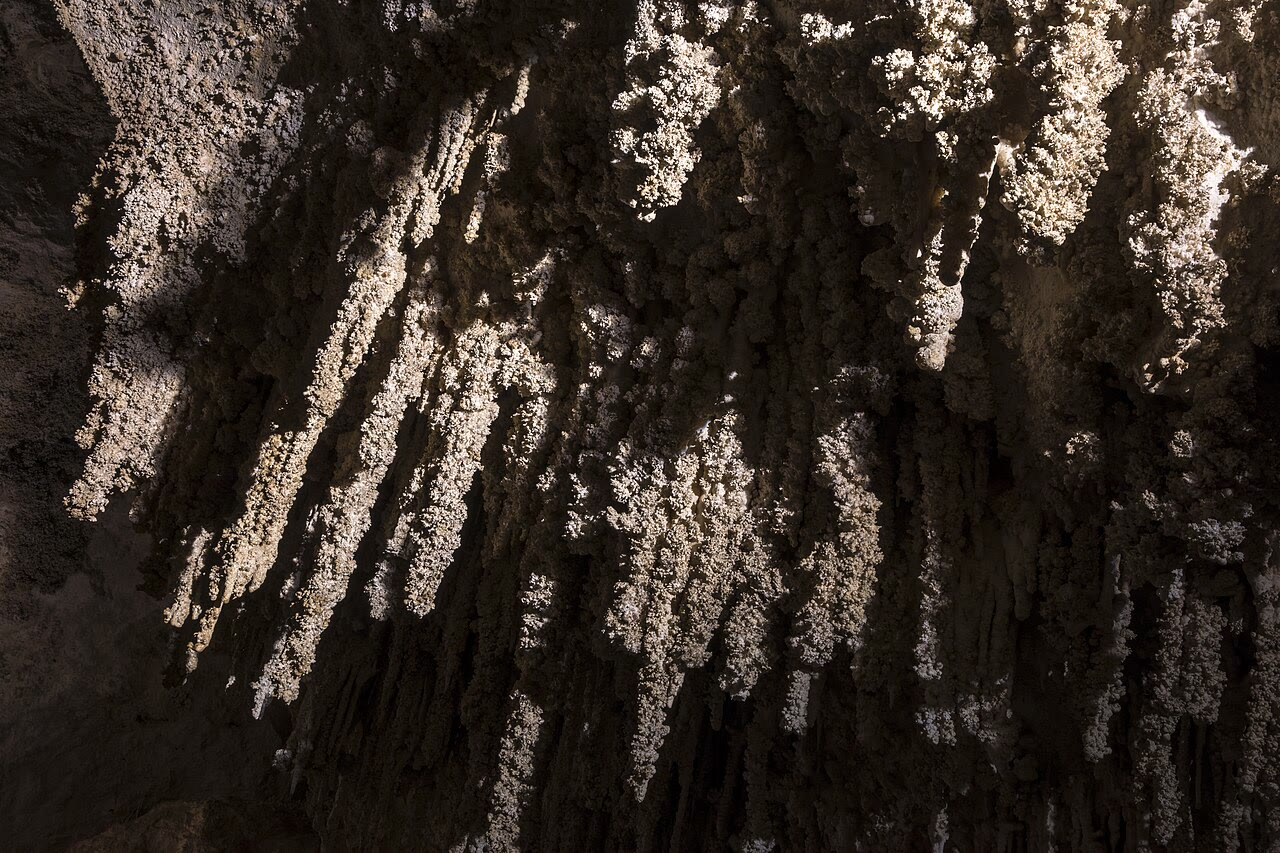
\includegraphics[width=\linewidth]{images/book1/g9-stalactites.jpg}
\end{minipage}\hfill
\begin{minipage}[c]{0.46\linewidth}\raggedright
{\small Stalactites hanging under a large block of \omterm{def:g3:stones-pebbles-sand:rock}{rock} in Carlsbad Cavern,
New Mexico, a \omterm{def:g9:landforms:karst}{cave} dissolved in limestone. Each one grew drop by drop from
water seeping through the \omterm{def:g3:stones-pebbles-sand:rock}{rock} above. National Park Service, 2018 (public
domain, via Wikimedia Commons).}
\end{minipage}
% ledger: commons:carlsbad-stalactites, nps:speleothems
\label{fig:g9:landforms:stalactites}
\end{omfigure}

\omterm{def:g9:landforms:karst}{Karst} country holds much water underground, but it flows fast through the
open cracks and is hardly filtered: whatever is spilled on the ground can
reach a \omterm{def:g6:water-underground:spring}{spring} quickly. And where the \omterm{def:g3:stones-pebbles-sand:rock}{rock} below has been dissolved, the
ground can sink or collapse: where people live, a \omterm{def:g9:landforms:karst}{sinkhole} that opens
suddenly can swallow roads and houses.
% ledger: nps:karst, usgs:sinkholes

\section{Reading a landscape}

Every \omterm{def:g1:landscapes-around-us:landform}{landform} is a clue. Its shape tells which agent made it; the agent
tells which process was at work, \omterm{def:g5:water-shapes-the-land:erosion}{erosion} or \omterm{def:g5:water-shapes-the-land:deposition}{deposition}; and the process
often tells something about the \omterm{def:g3:stones-pebbles-sand:rock}{rock} or the loose material underneath.

\begin{method}[Reading a landform]
\begin{enumerate}
  \item \textbf{Shape.} Describe the \omterm{def:g1:landscapes-around-us:landform}{landform}: a ridge, a hollow, a steep
        face, a flat shelf; its size; which way it points.
  \item \textbf{Agent and process.} Decide which agent made it (a \omterm{def:g1:landscapes-around-us:water}{river},
        ice, the wind, the \omterm{def:g2:water-on-earth:ocean}{sea}, dissolving water) and whether it was carved
        (\omterm{def:g5:water-shapes-the-land:erosion}{erosion}) or built (\omterm{def:g5:water-shapes-the-land:deposition}{deposition}).
  \item \textbf{Material.} Say what it is made of, or what the \omterm{def:g3:stones-pebbles-sand:rock}{rock} below
        is likely to be: loose \omterm{def:g3:stones-pebbles-sand:sand}{sand}, \omterm{def:g3:stones-pebbles-sand:pebble}{pebbles}, limestone, hard or soft \omterm{def:g3:stones-pebbles-sand:rock}{rock}.
\end{enumerate}
\end{method}

\begin{center}
{\small
\begin{tabular}{|>{\raggedright\arraybackslash}p{4.6cm}|>{\raggedright\arraybackslash}p{2.6cm}|>{\raggedright\arraybackslash}p{2.2cm}|>{\raggedright\arraybackslash}p{2.6cm}|}
\hline
shape & agent & process & material \\
\hline
crescent-shaped \omterm{def:g1:landscapes-around-us:landform}{hills} of \omterm{def:g3:stones-pebbles-sand:sand}{sand} & wind & \omterm{def:g5:water-shapes-the-land:deposition}{deposition} & loose \omterm{def:g3:stones-pebbles-sand:sand}{sand} \\
a vertical \omterm{def:g3:stones-pebbles-sand:rock}{rock} face above a flat \omterm{def:g3:stones-pebbles-sand:rock}{rock} shelf & \omterm{def:g2:water-on-earth:ocean}{sea} & \omterm{def:g5:water-shapes-the-land:erosion}{erosion} & \omterm{def:g3:stones-pebbles-sand:rock}{rock} (soft \omterm{def:g3:stones-pebbles-sand:rock}{rock} retreats fast) \\
a narrow ridge of \omterm{def:g3:stones-pebbles-sand:sand}{sand} across a bay & \omterm{def:g2:water-on-earth:ocean}{sea} (\omterm{def:g9:landforms:beach}{longshore drift}) & \omterm{def:g5:water-shapes-the-land:deposition}{deposition} & \omterm{def:g3:stones-pebbles-sand:sand}{sand} or \omterm{def:g3:stones-pebbles-sand:pebble}{pebbles} \\
hollows in fields, streams that vanish & dissolving water & dissolution & limestone \\
a \omterm{def:g8:ice-on-earth:glacial-landforms}{U-shaped valley} & ice & \omterm{def:g5:water-shapes-the-land:erosion}{erosion} & any \omterm{def:g3:stones-pebbles-sand:rock}{rock} \\
a fan of \omterm{def:g3:stones-pebbles-sand:sand}{mud} at a \omterm{def:g1:landscapes-around-us:water}{river} \omterm{def:g5:water-shapes-the-land:source-mouth}{mouth} & \omterm{def:g1:landscapes-around-us:water}{river} & \omterm{def:g5:water-shapes-the-land:deposition}{deposition} & \omterm{def:g3:stones-pebbles-sand:sand}{mud} and \omterm{def:g3:stones-pebbles-sand:sand}{sand} \\
\hline
\end{tabular}}
\end{center}

\begin{example}[A walk on a plateau]
On a high grassy plateau, there is no stream at all, although it \omterm{def:g4:clouds-rain-snow:precipitation}{rains}
often. The fields are dotted with round hollows a few metres across, and in
the \omterm{def:g1:landscapes-around-us:landform}{valley} below a powerful \omterm{def:g6:water-underground:spring}{spring} gushes out of the foot of a \omterm{def:g3:stones-pebbles-sand:rock}{rock} face.
\emph{Shape}: hollows, no streams on the surface, a \omterm{def:g6:water-underground:spring}{spring} lower down.
\emph{Agent and process}: water dissolving the \omterm{def:g3:stones-pebbles-sand:rock}{rock} and flowing
underground. \emph{Material}: the plateau is most likely limestone, and
the hollows are \omterm{def:g9:landforms:karst}{sinkholes}. A drop of dilute acid on a loose piece of the
\omterm{def:g3:stones-pebbles-sand:rock}{rock}, put by the teacher, would fizz.
\end{example}
% ledger: nps:karst, usgs:sinkholes

\section{Exercises}

\begin{exercise}[$\star$]\label{exo:g9:landforms:1}
Which agent made each \omterm{def:g1:landscapes-around-us:landform}{landform}: the wind, the \omterm{def:g2:water-on-earth:ocean}{sea}, a \omterm{def:g1:landscapes-around-us:water}{river}, ice, or water
dissolving the \omterm{def:g3:stones-pebbles-sand:rock}{rock}? (a) A crescent-shaped \omterm{def:g1:landscapes-around-us:landform}{hill} of \omterm{def:g3:stones-pebbles-sand:sand}{sand} in a \omterm{def:g5:weather-and-climate:desert}{desert}.
(b) A \omterm{def:g9:landforms:karst}{cave} full of stalactites. (c) A long ridge of \omterm{def:g3:stones-pebbles-sand:pebble}{pebbles} across the
mouth of a bay. (d) A \omterm{def:g8:ice-on-earth:glacial-landforms}{U-shaped valley} with a \omterm{def:g8:ice-on-earth:glacial-landforms}{moraine} at its end. (e) A
vertical chalk face with a flat \omterm{def:g3:stones-pebbles-sand:rock}{rock} shelf at its foot. (f) A \omterm{def:g5:water-shapes-the-land:delta}{delta}.
\end{exercise}

\begin{exercise}[$\star$]\label{exo:g9:landforms:2}
Give the word for each description. (a) The slow rise of the \omterm{def:g3:stones-pebbles-sand:rock}{rocks} and the
ground of a region. (b) The steep side of a \omterm{def:g9:landforms:dune}{dune}, away from the wind.
(c) A hole in the ground formed where the \omterm{def:g3:stones-pebbles-sand:rock}{rock} below has dissolved or a
\omterm{def:g9:landforms:karst}{cave} roof has collapsed. (d) The movement of \omterm{def:g3:stones-pebbles-sand:sand}{sand} and \omterm{def:g3:stones-pebbles-sand:pebble}{pebbles} along the
shore. (e) A \omterm{def:g1:landscapes-around-us:landscape}{landscape} shaped by water dissolving limestone.
\end{exercise}

\begin{exercise}[$\star$]\label{exo:g9:landforms:3}
True or false? Correct the false sentences. (a) The horns of a crescent
\omterm{def:g9:landforms:dune}{dune} point towards the wind. (b) The slope of a \omterm{def:g9:landforms:dune}{dune} facing the wind is
gentle. (c) A \omterm{def:g9:landforms:dune}{dune} moves because the wind lifts it all at once. (d) \omterm{def:g9:landforms:dune}{Dunes}
form more easily where few plants grow.
\end{exercise}

\begin{exercise}[$\star$]\label{exo:g9:landforms:4}
Put these steps of the retreat of a \omterm{def:g2:water-on-earth:ocean}{sea} \omterm{def:g9:landforms:cliff}{cliff} in order. (a) The waves break
up the fallen blocks and carry them away. (b) The waves cut a notch at the
foot of the \omterm{def:g9:landforms:cliff}{cliff}. (c) The \omterm{def:g9:landforms:cliff}{cliff} face now stands further inland, and the
flat platform in front of it is a little wider. (d) The \omterm{def:g3:stones-pebbles-sand:rock}{rock} above the
notch overhangs. (e) The overhang falls.
\end{exercise}

\begin{exercise}[$\star\star$]\label{exo:g9:landforms:5}
% ledger: nps:whsa-migration (6 and 3 m a year)
Seen from an aircraft, the crescent \omterm{def:g9:landforms:dune}{dunes} of a \omterm{def:g5:weather-and-climate:desert}{desert} all have their horns
pointing to the east. (a) From which direction does the wind blow? (b) On
which side of each \omterm{def:g9:landforms:dune}{dune} is the \omterm{def:g9:landforms:dune}{slip face}? (c) A road runs \qty{60}{m} east
of one of the \omterm{def:g9:landforms:dune}{dunes}. The \omterm{def:g9:landforms:dune}{dune} moves \qty{6}{m} a year. In how many years
will its foot reach the road? (d) A larger \omterm{def:g9:landforms:dune}{dune} moves only \qty{3}{m} a
year. Why do larger \omterm{def:g9:landforms:dune}{dunes} move more slowly?
\end{exercise}

\begin{exercise}[$\star\star$]\label{exo:g9:landforms:6}
% ledger: sdnp:birling, nt:birling-2014
The chalk \omterm{def:g9:landforms:cliff}{cliffs} of a \omterm{def:g1:landscapes-around-us:water}{coast} retreat by up to about \qty{1}{m} a year. In
the winter of 2014, they lost as much as they usually lose in seven years,
in only two months. (a) At \qty{1}{m} a year, how much is lost in seven
years? (b) Two months is what fraction of a year? (c) How many times faster
than usual did the \omterm{def:g9:landforms:cliff}{cliffs} retreat during those two months? (d) Explain,
using the notch and the overhang, why a \omterm{def:g9:landforms:cliff}{cliff} retreats in jumps rather
than smoothly.
\end{exercise}

\begin{exercise}[$\star\star$]\label{exo:g9:landforms:7}
A straight \omterm{def:g1:landscapes-around-us:water}{coast} runs west--east, with the \omterm{def:g2:water-on-earth:ocean}{sea} to the south. The waves
come from the south-west. (a) In which direction does the \omterm{def:g9:landforms:beach}{longshore drift}
carry the \omterm{def:g3:stones-pebbles-sand:sand}{sand}? (b) Draw the zigzag path of a \omterm{def:g3:stones-pebbles-sand:pebble}{pebble} over three waves,
labelling the stroke up the \omterm{def:g9:landforms:beach}{beach} and the stroke back down. (c) At its east
end the \omterm{def:g1:landscapes-around-us:water}{coast} turns north into a bay. What \omterm{def:g1:landscapes-around-us:landform}{landform} is likely to grow
there? (d) Why does \omterm{def:g3:stones-pebbles-sand:sand}{mud} settle behind it?
\end{exercise}

\begin{exercise}[$\star\star$]\label{exo:g9:landforms:8}
(a) What makes rainwater slightly acidic? (b) Why are there \omterm{def:g9:landforms:karst}{caves} in
limestone but hardly any in granite? (c) Why do the \omterm{def:g9:landforms:karst}{caves} follow the cracks
and layers of the \omterm{def:g3:stones-pebbles-sand:rock}{rock}? (d) Give two ways a \omterm{def:g9:landforms:karst}{sinkhole} can form.
\end{exercise}

\begin{exercise}[$\star\star$]\label{exo:g9:landforms:9}
(a) Explain why calcite comes out of a drop of water hanging from a \omterm{def:g9:landforms:karst}{cave}
roof. (b) Why do stalagmites have no hollow tube inside, unlike young
stalactites? (c) Suppose a stalactite has grown \qty{0.1}{mm} a year (an
invented rate: real rates vary a lot). How many years has it taken to grow
\qty{30}{cm}? Write the answer in scientific notation.
\end{exercise}

\begin{exercise}[$\star\star$]\label{exo:g9:landforms:10}
% ledger: usgs:himalaya, sdnp:birling
The Tibetan Plateau rose about \qty{4600}{m} in about 10~million years.
(a) Compute the average \omterm{def:g9:landforms:uplift}{uplift} in metres per year, in scientific notation,
then in millimetres per year. (b) Suppose \omterm{def:g5:water-shapes-the-land:erosion}{erosion} removes \qty{0.2}{mm} a
year from the plateau (an invented figure). By how much does the plateau
rise each year? (c) A chalk \omterm{def:g9:landforms:cliff}{cliff} retreats about \qty{1}{m} a year. How many
times faster is that than the \omterm{def:g9:landforms:uplift}{uplift} of (a)? (d) Why can a slow \omterm{def:g9:landforms:uplift}{uplift}
still build a high plateau?
\end{exercise}

\begin{exercise}[$\star\star\star$]\label{exo:g9:landforms:11}
Read each \omterm{def:g1:landscapes-around-us:landscape}{landscape} with the method of the chapter (shape, agent and
process, material). (a) In a dry country, long lines of \omterm{def:g3:stones-pebbles-sand:sand}{sand} \omterm{def:g1:landscapes-around-us:landform}{hills}, each
shaped like a crescent, with a steep side facing south-east. (b) At the
foot of a white \omterm{def:g9:landforms:cliff}{cliff}, a flat \omterm{def:g3:stones-pebbles-sand:rock}{rock} shelf covered with seaweed appears at
low tide. (c) On a wide plateau of pale \omterm{def:g3:stones-pebbles-sand:rock}{rock}, a stream flows across a field
and disappears into a hole; a \omterm{def:g6:water-underground:spring}{spring} gushes out of a \omterm{def:g1:landscapes-around-us:landform}{valley} side
\qty{2}{km} away.
\end{exercise}

\begin{exercise}[$\star\star\star$]\label{exo:g9:landforms:12}
% ledger: nps:whsa-migration, nmt:barchan, nps:aeolian
In a \omterm{def:g9:landforms:dune}{dune} field, the small \omterm{def:g9:landforms:dune}{dunes} at the upwind edge move up to \qty{6}{m} a
year; a little further on, the \omterm{def:g9:landforms:dune}{dunes}, 6 to \qty{10}{m} high, move about
\qty{3}{m} a year. A track crosses the field \qty{45}{m} downwind of a \omterm{def:g9:landforms:dune}{dune}
of each kind. (a) After how many years does each \omterm{def:g9:landforms:dune}{dune} reach the track?
(b) \omterm{def:g9:landforms:dune}{Dunes} driven by strong winds can travel more than \qty{100}{m} in a
year. How long would such a \omterm{def:g9:landforms:dune}{dune} take to cover the same distance? (c) Name
one way to slow the \omterm{def:g9:landforms:dune}{dunes} down, and explain how it works.
\end{exercise}

\section{Problem: The cliff and the coast road}

\begin{problem}[{Weekend problem --- a coast road runs behind a retreating
chalk cliff; the final answer is the year the cliff edge would reach the
road at the measured rate}]
\label{pb:g9:landforms:1}
% ledger: (invented region: exercise data, figdata/grade-9/cliff_retreat.py; the rate is kept within sdnp:birling, the storm winter recalls nt:birling-2014)
A \omterm{def:g1:landscapes-around-us:water}{coast} road runs along the top of chalk \omterm{def:g9:landforms:cliff}{cliffs}. Every few years, a survey
team measures the distance from the road to the \omterm{def:g9:landforms:cliff}{cliff} edge along the same
line, from fixed markers set well back from the edge, never at the edge
itself. Here are their measurements.

\begin{center}
{\small
\begin{tabular}{|l|c|c|c|c|c|c|c|}
\hline
year & 2004 & 2008 & 2012 & 2014 & 2016 & 2020 & 2024 \\
\hline
distance from the road to the edge (m) & 46.0 & 43.1 & 41.0 & 36.2 & 35.5 & 33.0 & 30.4 \\
\hline
\end{tabular}}
\end{center}

\noindent\textbf{Part I --- The measurements.}\par\nopagebreak
\begin{enumerate}[beginpenalty=10000]
  \item By how many metres did the \omterm{def:g9:landforms:cliff}{cliff} edge move closer to the road
        between 2004 and 2024?
  \item Compute the average rate of retreat over these 20 years, in metres
        per year.
  \item Between which two surveys did the edge retreat fastest? Compute the
        rate over that interval.
  \item How many times faster than the average is it? Suggest what
        happened during that interval.
\end{enumerate}

\begin{omfigure}
\begin{tikzpicture}
\begin{axis}[omrecord, width=11cm, height=4.6cm, xmin=2000, xmax=2070,
  ymin=0, ymax=50, xtick={2000,2010,...,2070}, ytick={0,10,...,50},
  x tick label style={/pgf/number format/1000 sep={}},
  xlabel={year}, ylabel={distance to the road (m)}]
  \addplot[omWarm, thick, mark=*, mark size=1.8pt] table[x=year, y=dist_m] {figdata/out/grade-9-cliff_retreat.dat};
\end{axis}
\end{tikzpicture}

{\small The survey: distance from the \omterm{def:g1:landscapes-around-us:water}{coast} road to the \omterm{def:g9:landforms:cliff}{cliff} edge (exercise
data).}
\label{fig:g9:landforms:survey}
\end{omfigure}

\noindent\textbf{Part II --- The rate.}\par\nopagebreak
\begin{enumerate}[resume, beginpenalty=10000]
  \item Write the average rate in centimetres per year, then in metres per
        century.
  \item On a real chalk \omterm{def:g1:landscapes-around-us:water}{coast}, the \omterm{def:g9:landforms:cliff}{cliffs} retreat by up to about a metre a
        year. Is this \omterm{def:g9:landforms:cliff}{cliff}'s retreat of the same size?
  \item A lighthouse on such a \omterm{def:g1:landscapes-around-us:water}{coast} was once moved \qty{17}{m} back from
        the edge. At this \omterm{def:g9:landforms:cliff}{cliff}'s average rate, how many years of retreat
        does \qty{17}{m} represent?
  \item Why is the rate measured over 20 years a better guide to the
        future than the rate measured over two years?
\end{enumerate}

\noindent\textbf{Part III --- The road.}\par\nopagebreak
\begin{enumerate}[resume, beginpenalty=10000]
  \item The road is to be moved before the edge comes within \qty{10}{m} of
        it. In which year, at the average rate, will that be?
  \item If stormier winters doubled the rate, in which year would the edge
        reach the road?
  \item Why does the survey team take its measurements from markers set
        well back from the edge?
  \item At the average rate, in which year would the \omterm{def:g9:landforms:cliff}{cliff} edge reach the
        road?
\end{enumerate}
\end{problem}
